\documentclass[a4paper,12pt]{article}
\usepackage[russian,ukrainian,english]{babel}
\usepackage[T2A,T1]{fontenc}
\usepackage[utf8]{inputenc}

\usepackage{hyperref}
\usepackage{graphics}
\usepackage{graphicx}
\usepackage{listings}
\usepackage{bera}
\usepackage{listings}
\usepackage{xcolor}

\pagestyle{headings}
 
\colorlet{punct}{red!60!black}
\definecolor{background}{HTML}{EEEEEE}
\definecolor{delim}{RGB}{20,105,176}
\colorlet{numb}{magenta!60!black} 
 
\lstdefinelanguage{json}{
    basicstyle=\normalfont\ttfamily,
    numbers=left,
    numberstyle=\scriptsize,
    stepnumber=1,
    numbersep=8pt,
    showstringspaces=false,
    breaklines=true,
    frame=lines,
    backgroundcolor=\color{background},
    literate=
     *{0}{{{\color{numb}0}}}{1}
      {1}{{{\color{numb}1}}}{1}
      {2}{{{\color{numb}2}}}{1}
      {3}{{{\color{numb}3}}}{1}
      {4}{{{\color{numb}4}}}{1}
      {5}{{{\color{numb}5}}}{1}
      {6}{{{\color{numb}6}}}{1}
      {7}{{{\color{numb}7}}}{1}
      {8}{{{\color{numb}8}}}{1}
      {9}{{{\color{numb}9}}}{1}
      {:}{{{\color{punct}{:}}}}{1}
      {,}{{{\color{punct}{,}}}}{1}
      {\{}{{{\color{delim}{\{}}}}{1}
      {\}}{{{\color{delim}{\}}}}}{1}
      {[}{{{\color{delim}{[}}}}{1}
      {]}{{{\color{delim}{]}}}}{1},
}
 
 \lstdefinestyle{DOS} {
    backgroundcolor=\color{black},
    basicstyle=\scriptsize\color{white}\ttfamily
}

 
 \title{Data Wrangle OpenStreetMaps Data}
\date{February 3, 2015}
\author{Oleksii Renov}
        
\begin{document}
\maketitle

\section*{Choosing map area}
 
Choosing map area is very simple for me. I live in Kiev, Ukraine. So i hadn't got another choice. As the very first step I need minimum and maximum longitude and latitude. For this task I'd gone to \url{http://openstreetmap.org} in the search field I'd typed Kiev and choose the second link. I've the following web page in my browser.\par
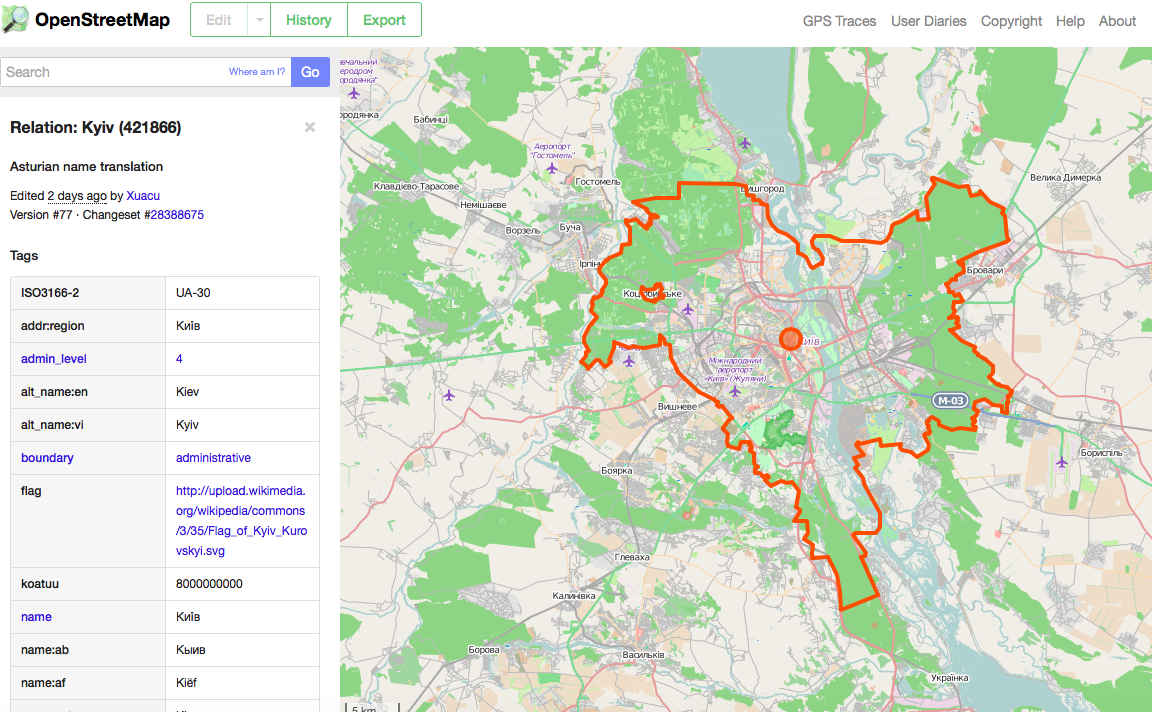
\includegraphics[scale=0.35]{keivinit.png}  
\par
I've done some zomming and choose next latitude and longitude parameters in my case:
\begin{itemize}
\item minimum latitude = 29.9048;
\item maximum latitude = 50.0986;
\item minimum longitude = 31.1600;
\item maximum longitude = 50.7052.
\end{itemize}
 
 Next step is to download my dataset. I've gone in \url{http://overpass-api.de/query_form.html}, where i can past some queries to download data what i need.\par

 My query is next:
 \begin{lstlisting}
(node(29.9048, 50.0986, 31.1600, 50.7052);<;);out;
\end{lstlisting}
Anyway there is exists numbers of variants loading data. One of them is simply go to this url \url{ http://overpass-api.de/api/map?bbox=29.9048,50.0986,31.1600,50.7052}. The xml file which I've already downloaded is very big, near 250mb. In my usual work i've chance working with xml, and files near 1mb is very hard to analyze. Let's move to processing this dataset.

\section*{Process Dataset}

As very first step, let's check what tags are in our dataset. Also would be helpful to check for attributes. Let's start from tags. 

\begin{lstlisting}[language=json,firstnumber=1]
{'bounds': 1,
 'member': 75124,
 'meta': 1,
 'nd': 1316743,
 'node': 1079619,
 'note': 1,
 'osm': 1,
 'relation': 5016,
 'tag': 417122,
 'way': 153102}
\end{lstlisting}
Next json is corresponded to tag attributes.
\begin{lstlisting}[language=json,firstnumber=1]
{'changeset': 1237737,
 'generator': 1,
 'id': 1237737,
 'k': 417122,
 'lat': 1079619,
 'lon': 1079619,
 'maxlat': 1,
 'maxlon': 1,
 'minlat': 1,
 'minlon': 1,
 'osm_base': 1,
 'ref': 1391867,
 'role': 75124,
 'timestamp': 1237737,
 'type': 75124,
 'uid': 1237737,
 'user': 1237737,
 'v': 417122,
 'version': 1237738}
\end{lstlisting}
First of all i would like to notice, that 'k' is key and 'v' is value. There are equal number of keys and values what is obvious. But it isn't clear what this keys are holding. I would like to explore more details and understand what keys and values have the most frequency in my dataset. In my opinion top 10 would be perfect for start.
\begin{lstlisting}[language=json,firstnumber=1]
{('surface', 9780),
 ('amenity', 9919),
 ('name:en', 10396),
 ('name:uk', 10646),
 ('name:ru', 12823),
 ('addr:street', 14084),
 ('name', 23862),
 ('addr:housenumber', 30646),
 ('highway', 67770),
 ('building', 73142)}
\end{lstlisting}
There are few nice things here. Due to Ukraine history we have official street name in ukrainian, unofficial russian and english names. For convinience I'm going to analyze here only international names. Let's check some values for key 'amenity'. For me it's very interesting.
\begin{lstlisting}[language=json,firstnumber=1]
 {('place_of_worship', 300),
 ('bench', 331),
 ('atm', 374),
 ('kindergarten', 419),
 ('fuel', 425),
 ('restaurant', 514),
 ('cafe', 520),
 ('school', 543),
 ('pharmacy', 566),
 ('bank', 770),
 ('parking', 1812)}
\end{lstlisting}
Let's try to analyze values, we've chosen three regular expressions to check text for lowercase, problem strings and others. Especially we would like to explore data with bad keys. 
\begin{lstlisting}[language=json,firstnumber=1]
{'lower': 258569,
'lower_colon': 163,
'other': 157676,
'problemchars': 714}
\end{lstlisting}
Let's take a loot at keys which values contain problem characters.
\begin{lstlisting}[language=json,firstnumber=1]
{'building:color': 2,
'contact:phone': 40,
'phone': 558,
'roof:colour': 19,
'wheelchair': 1}
\end{lstlisting}
There are exists more keys, but i want to point at not standartized phone numbers for this dataset. Let's look at them.
\begin{lstlisting}[language=json, firstnumber=1]
'+3-8-093-207-31-01, +3-8-067-838-47-64, +3-8-067-401-75-61'
 '+380 44 251-34-34',
 '+38(098)-109-5001',
 '+380 44 490 20 30',
 '+38 067 500 81 89',
\end{lstlisting}
Oh.. There are lots of phone numbers in different formats. I'm going to create one format for phone number for this dataset. It's can will be a list of phones even list can have only size equal to 1.\par
From wikipedia \url{http://en.wikipedia.org/wiki/Telephone_numbers_in_Ukraine} i've read that typical Ukrainian phone numbers is:
\begin{itemize}
\item +380 xx xxx-xx-xx (general phone numbers);
\end{itemize}
I've written script for this preprocessing, before converting data in JSON and loading data to MongoDB. Next little python script handle different data formats and standartize them.
\begin{lstlisting}[language=python, firstnumber=1, caption={Phone standartization}]
def convertPhone(phone):
    # First step i'm going to remove all non number characters
    phone = re.sub('\D', '', phone)
    if len(phone) == 10:
        phone = "+38" + phone
    elif len(phone) == 7:
        phone = "+38044" + phone
    elif len(phone) == 12:
        phone = "+" + phone
    elif len(phone) == 11:
        phone = "+3" + phone
    elif len(phone) == 9:
        phone = "+380" + phone

    if len(phone) == 13:
        phone = phone[0:4] + ' ' + phone[4:6] + ' ' + phone[6:9] +
         '-' + phone[9:11] + '-' + phone[11:13]
    return phone
\end{lstlisting} 
Results of transformation:
\begin{itemize}
\item '+380(44)593-12-06' to '+380 44 593-12-06';
\item ' +380-44-599-60-82' to '+380 44 599-60-81';
\item '3317730' to '+380 44 331-77-30'.
\end{itemize}
Nice results. Let's audit streets names. Ukraine has next common street types:\par
expected = ["\foreignlanguage{russian}{вулиця}",  "\foreignlanguage{russian}{бульвар}", "\foreignlanguage{russian}{проспект}", "\foreignlanguage{russian}{узвіз}", "\foreignlanguage{russian}{площа}", "\foreignlanguage{russian}{провулок}", "\foreignlanguage{russian}{шосе}", "\foreignlanguage{russian}{набережна}", "\foreignlanguage{russian}{тупик}"," \foreignlanguage{russian}{дорога}", "\foreignlanguage{russian}{проїзд}", "\foreignlanguage{russian}{шлях}"]\par
And next mapping:\par
mapping = [ "\foreignlanguage{russian}{вул.}": "\foreignlanguage{russian}{вулиця}",\par
            "\foreignlanguage{russian}{пр}.": "\foreignlanguage{russian}{проспект}",\par
            "\foreignlanguage{russian}{пл.}" : "\foreignlanguage{russian}{площа}",\par
            '\foreignlanguage{russian}{пров.}' : '\foreignlanguage{russian}{провулок}'\par
]
Next step is converting xml to json and loading data in mongodb. I've used data.py for creating json. Then I've started mongo shell navigate to folder which contain map.json. I've used mongoimport tool:
\begin{lstlisting}[style=DOS]
 mongoimport -d test -c kiev map.json
\end{lstlisting}
\subsection*{Data Overview}
Let explore how number of documents in our db and it size.
\begin{lstlisting}[caption={Size and number of documents in db.},style=DOS]
> show dbs
admin     (empty)
examples  0.078GB
local     0.078GB
osm       (empty)
test      0.953GB
> use test
switched to db test
> db.kiev.find().count()
1232721
\end{lstlisting}
Next step is to find number of 'ways', 'nodes' and uniques users.
\begin{lstlisting}[style=DOS,caption={Basic statistics}]
> db.kiev.find({"type":"node"}).count()
1079585
> db.kiev.find({"type":"way"}).count()
152949
> db.kiev.distinct('created.user').length
1303
\end{lstlisting}

Let find more interesting statistics: number of cafes, cinemas, banks and fuels.
\begin{lstlisting}[style=DOS]
> db.kiev.find({'amenity':'cafe'}).count()
520
> db.kiev.find({'amenity':'cinema'}).count()
47
> db.kiev.find({'amenity':'bank'}).count()
770
> db.kiev.find({'amenity':'fuel'}).count()
422
\end{lstlisting}
\section*{Additional Data Overview}
Let's find top 10 amenities.
\begin{lstlisting}[style=DOS]
> db.kiev.aggregate([{"$match":{"amenity":{"$exists":1}}}, {"$group":{"_id":"$amenity",
 "count":{"$sum":1}}}, {"$sort" : {"count" : -1}}, {"$limit" : 10}])
{ "_id" : "parking", "count" : 1784 }
{ "_id" : "bank", "count" : 770 }
{ "_id" : "pharmacy", "count" : 566 }
{ "_id" : "cafe", "count" : 520 }
{ "_id" : "school", "count" : 517 }
{ "_id" : "restaurant", "count" : 514 }
{ "_id" : "fuel", "count" : 422 }
{ "_id" : "kindergarten", "count" : 405 }
{ "_id" : "atm", "count" : 374 }
{ "_id" : "bench", "count" : 331 }
\end{lstlisting}
Let's explore to 10 banks in Kyiv.
\begin{lstlisting}[style=DOS]
> db.kiev.aggregate([{"$match":{"amenity":"bank"}}, 
{"$group":{"_id":"$name", "count":{"$sum":1}}}, 
{"$sort" : {"count" : -1}}, {"$limit" : 10}])
{ "_id" : "OschadnyBank", "count" : 87 }
{ "_id" : "PrivatBank", "count" : 86 }
{ "_id" : "UkrSibBank", "count" : 51 }
{ "_id" : null, "count" : 50 }
{ "_id" : "Raifaisen Bank Aval", "count" : 21 }
{ "_id" : "UniCredit Bank", "count" : 16 }
{ "_id" : "PraveksBank", "count" : 16 }
{ "_id" : "CityCommerce Bank", "count" : 15 }
{ "_id" : "Sberbank Russia", "count" : 14 }
{ "_id" : "Delta Bank", "count" : 13 }
\end{lstlisting}
All religions in city based on openstreetmaps data.
\begin{lstlisting}[style=DOS]
> db.kiev.aggregate([{"$match":{"amenity":"place_of_worship"}},
 {"$group":{"_id":"$religion","count":{"$sum":1}}}, 
 {"$sort":{"count":-1}},{"$limit":1}])
{ "_id" : "christian", "count" : 275 }
\end{lstlisting}
How many traffic signals in Kiev based on OSM data?
\begin{lstlisting}{style=DOS}
> db.kiev.find({"highway":"traffic_signals"}).count()
854
\end{lstlisting}
Let's find top 10 combinations of website and amenity.
\begin{lstlisting}[style=DOS]
> db.kiev.aggregate([{"$match": {"amenity":{"$exists":1}, "website":{"$exists":1}}}, 
{"$group": {"_id":{"amenity": "$amenity", "website":"$website"}, "count":{"$sum":1}}}, 
{"$sort":{"count":-1}}, {"$limit":10}])
{ "_id" : { "amenity" : "bank", "website" : "www.oschadnybank.com" }, "count" : 64 }
{ "_id" : { "amenity" : "bank", "website" : "www.ukrsibbank.com" }, "count" : 38 }
{ "_id" : { "amenity" : "bank", "website" : "http://www.citycommercebank.com/" }, "count" : 14 }
{ "_id" : { "amenity" : "bank", "website" : "www.deltabank.com.ua" }, "count" : 10 }
{ "_id" : { "amenity" : "bank", "website" : "http://www.oschadnybank.com" }, "count" : 9 }
{ "_id" : { "amenity" : "bank", "website" : "www.piraeusbank.ua" }, "count" : 7 }
{ "_id" : { "amenity" : "bank", "website" : "http://www.ukrsibbank.com" }, "count" : 7 }
{ "_id" : { "amenity" : "fast_food", "website" : "www.pizza-celentano.com" }, "count" : 6 }
{ "_id" : { "amenity" : "bank", "website" : "http://www.procreditbank.com.ua/" }, "count" : 5 }
{ "_id" : { "amenity" : "fast_food", "website" : "http://www.mcdonalds.ua" }, "count" : 5 }
\end{lstlisting}

\subsection*{Conclusion}
After this review of the data it’s obvious that the Kiev city area is incomplete, though I believe it has been well cleaned for the purposes of this exercise. It interests me to notice a fair amount of GPS data makes it into OpenStreetMap.org on account of users’ efforts, whether by scripting a map editing bot or otherwise. I've cleaned and standartized phone numbers and street names, also i've found that also should be standartized websites info. For me is very surprising to see, that the most frequent amenity is parking and bank (my hypothesis was shops or restaurant). I've found top ten banks in Kiev using OSM data. It's interesting to know that we 854 traffic signals in Kiev. This was great experience to work maps data.

\subsection*{List of Resources}
\begin{enumerate}
\item Openstreetmap. Url: \url{http://www.openstreetmap.org}
\item Overpass Api. Url: \url{http://wiki.openstreetmap.org/wiki/Overpass_API}
\item MongoDB Documentation. Url: \url{http://docs.mongodb.org/manual/core/document/}
\item Python Mongo Drivers. Url: \url{http://docs.mongodb.org/ecosystem/drivers/python/}
\item Unicode HowTo. Url:\url{https://docs.python.org/2/howto/unicode.html}
\end{enumerate}
\end{document}